\section{Approaches}
\subsection{Recurrent Neural Networks}

\begin{frame}{Preparation}
    \begin{enumerate}
        \item Fill all time stamps with no task with a complexity-free task
        \item Train a recurrent neural network (GRU or LSTM) to predict task complexity in the next time stamp
        \item Store the trained task complexity distribution to decide the number of allocated nodes. Suppose that a task with complexity $C$ is at cumulative distribution point $p$, then it is allocated
              $$\min\{\texttt{available\_nodes}, \texttt{total\_nodes}\times p\}.$$
    \end{enumerate}
\end{frame}

\begin{frame}{Training and Testing}
    We train a two-layer LSTM with a 64-dimensional fully connected layers during 300 epochs.
    \begin{figure}
        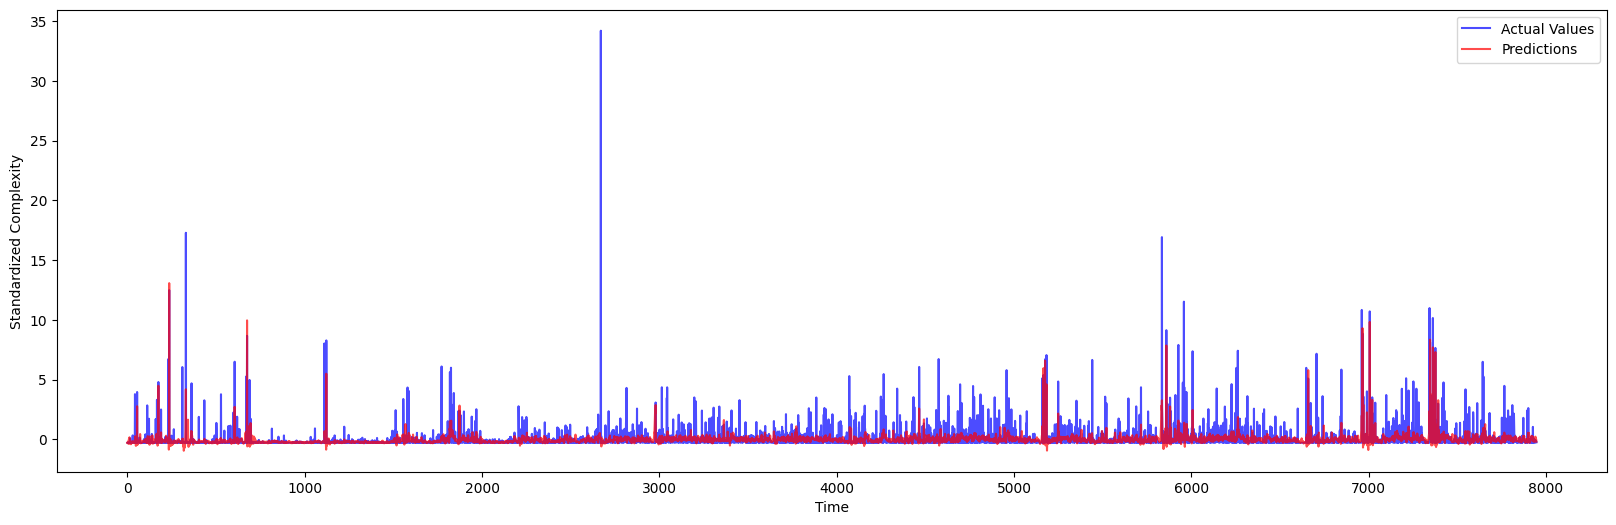
\includegraphics[width=0.9\textwidth]{img/train_accuracy.png}
        \caption{Model fit on the training data}
    \end{figure}
\end{frame}

\begin{frame}{Recurrent Neural Networks}
    \begin{figure}
        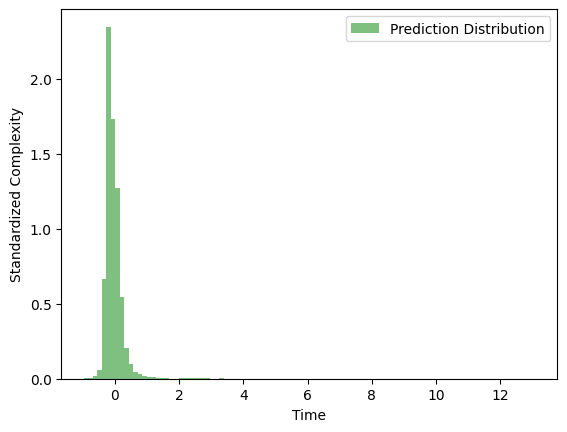
\includegraphics[width=0.5\textwidth]{img/complexity_ditribution.png}
        \caption{Complexity distribution}
    \end{figure}
\end{frame}

\begin{frame}{Recurrent Neural Networks}
    \begin{figure}
        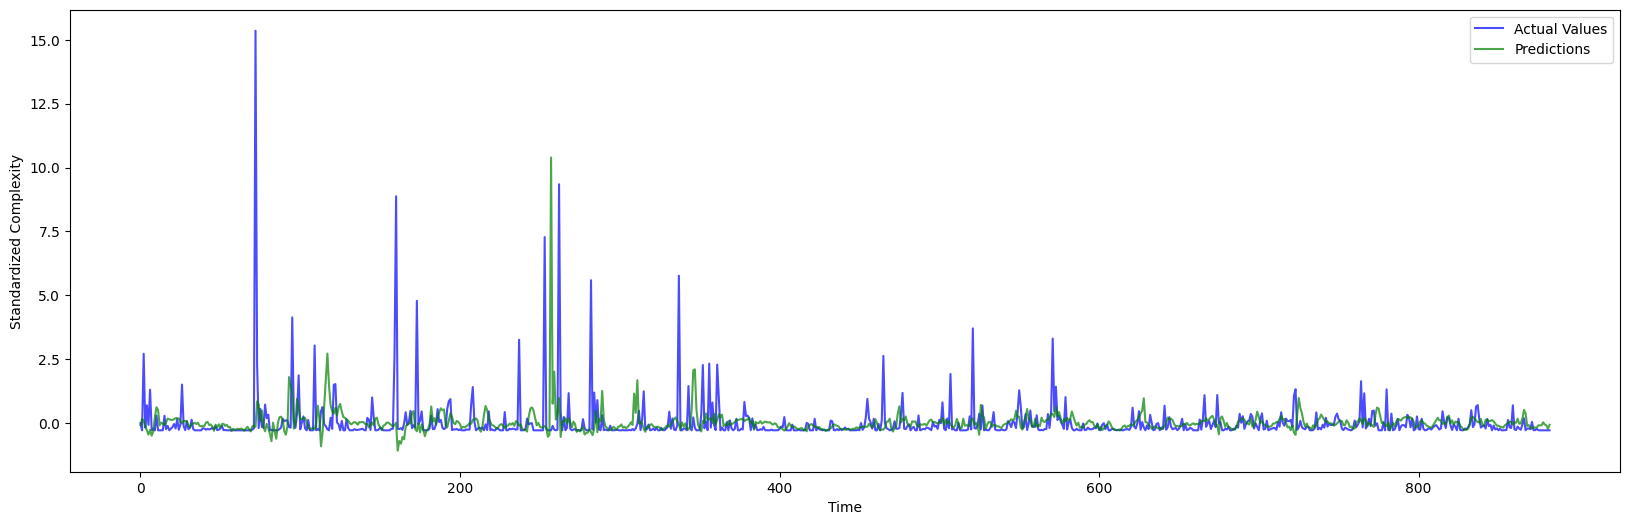
\includegraphics[width=0.9\textwidth]{img/test_accuracy.png}
        \caption{Prediction on the test data}
    \end{figure}
\end{frame}

\subsection{Deep Reinforcement Learning}

\begin{frame}{Deep Reinforcement Learning}
    \begin{itemize}
        \item Environment:
              \begin{itemize}
                  \item total tasks, total nodes
                  \item waiting tasks, available nodes
                  \item executing tasks, executed tasks
              \end{itemize}
        \item Observable states: available nodes, waiting queue (tasks along with waiting times)
        \item Actions: allocating $n \ge 0$ nodes based on available nodes
        \item Algorithms: Actor-Critic \footnotetext{Konda, Vijay, and John Tsitsiklis. "Actor-critic algorithms." Advances in neural information processing systems 12 (1999).} or Proximal Policy Optimization (PPO) \footnotetext{Schulman, John, et al. "Proximal policy optimization algorithms." arXiv preprint arXiv:1707.06347 (2017).}
    \end{itemize}
\end{frame}

\subsection{Comparison}
\begin{frame}
    We compare average waiting times of LSTM scheduler, PPO scheduler against common policies
    \begin{itemize}
        \item Linear scheduler: allocates $\min\{\ell, \texttt{available\_nodes}\}$ for each time stamp, where $\ell$ is a a constant.
        \item Stochastic scheduler: allocates $\min\{x, \texttt{available\_nodes}\}$ for each time stamp, where $x$ is the realization of a random variable $X$ with Poisson distribution.
    \end{itemize}

    LSTM and PPO schedulers take more time to simulate than common policies. For efficiency, PPO performs over two times better than common policies, while LSTM is slightly better.
\end{frame}